\section{Problem position} \label{position}

\paragraph{Notations.} 

Vectors and matrix are written in bold, only basic linear algebra is used. For instance, $x_n(t)$ stands for the value of the $n$-th node at time $t$, ${\bf x}_n$ for the whole values of the node along time, ${\bf x}(t)$ the whole values of the nodes at time $t$ and ${\bf x}$ all network values.

The Heaviside function writes $H(u)$ (considering $H(0) = 1/2$) and the sign function writes $sg(u) = 2 \, H(u) -1$:
\eqline{H(u) \deq \left\{\begin{array}{rl} 1 & \mbox{ if } u > 0 \\ 1/2 & \mbox{ if } u = 0 \\ 0 & \mbox{ if } u < 0. \\ \end{array} \right.}

Partial derivatives are written in compact form, e.g., $\partial_{x_n(t)} \, {\bf f}({\bf x})$ means $\frac{\partial {\bf f}({\bf x})}{\partial x_n(t)}$,
while $\partial_{x_n(t)\,x_{n'}(t')} \, {\bf f}({\bf x})$ means $\frac{\partial^2 {\bf f}({\bf x})}{\partial x_n(t) \,\partial x_{n'}(t')}$.

The notation $\delta_{\cal P}$ stands for $1$ is the property ${\cal P}$ is true and $0$ otherwise (e.g., $\delta_{2 > 1} = 1$).

Other notations are made explicit as soon as used.

\subsection*{A general recurrent architecture.}

\begin{figure}[!ht]
  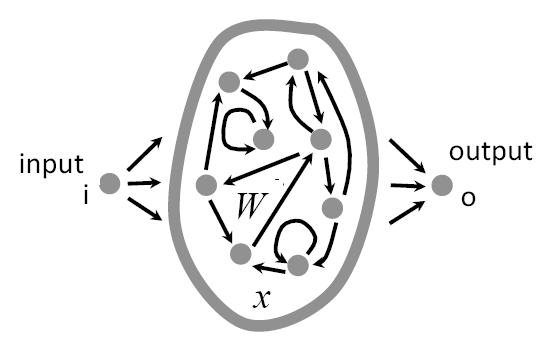
\includegraphics[width=0.8\textwidth]{img/recurrent-network}
  \caption{A General recurrent architecture maps a vectorial input sequence ${\bf i}(t)$ onto an output ${\bf o}(t)$, 
    via an internal state ${\bf x}(t)$ of hidden units. It is parameterized by a recurrent parameter matrix ${\bf W}$. 
    The dynamics is defined by the network recurrent equations.}
  \label{recurrent-network}
\end{figure}

As schematized in figure~\ref{recurrent-network}, we consider a recurrent network 
\eqline{x_n(t) = \Phi_{nt}\left(\cdots, x_{n'}(t'), \cdots, i_{m}(s), \cdots\right)}
with nodes of the form:
\begin{equation}\label{eq-recurrent}
\begin{array}{rcl} 
x_n(t) &=& \Phi_{n0t}\left(\cdots, x_{n'}(t'), \cdots, i_{m}(s), \cdots\right) \\ 
          &+& \sum_{d = 1}^{D_{n}} W_{nd} \, \Phi_{ndt}\left(\cdots, x_{n'}(t'), \cdots, i_{m}(s), \cdots\right) \\
o_n(t) &=& x_n(t), n < N_0 \\
 \end{array}
\end{equation} 
i.e., defined as a linear combination of some kernel $\Phi_{ndt}()$.
We show in Appendix~\ref{generality} that this a very general form
(e.g., including when considering the adjustment of unit parameters
that are not connection weights).

More precisely, equation~(\ref{eq-recurrent}) elements define:
 \\  -  $N$ nodes of value $x_{n}(t)$ indexed by $n \in \{0, N\{$, 
 \\  \hphantom{0.5cm} -  with a maximal state recurrent causal range of $R$ and with either,  
 \\  \hphantom{0.8cm} -  $t - R \leq t' < t$ (i.e., taking into account previous value up to $R$ time-steps in the past) or
 \\  \hphantom{0.8cm} -  $t' = t$ and $n < n'$ (i.e., taking into account present value, of subsequent nodes, in a causal way).
 \\  \hphantom{0.5cm} - while $N_0 \leq N$ of these nodes are output;
 \\  - $M$ input $i_{m}(s)$ indexed by $m \in \{0, M\{$, $t - S \leq  s < t$, 
 \\  - $1 + D_{n}$ predefined kernels $\Phi_{ndt}\left(\right)$ for each node, defining the network structure;
 \\  - $\sum_n D_n$ static adjustable weights $W_{nd}$, defining the network parameter.

\vphantom{1cm}

Considering equation~(\ref{eq-recurrent}) we notice that : \begin{itemize}

\item The distinction between output or hidden node is simply based on the fact that we can (or not) observe the $o_n(t)$ node value. Here, without loss of generality, output nodes are the $N_0 \leq N$ first ones.

\item Though, in order to keep compact notations, we mixed node with either 
 \\ \hphantom{0.2cm} - {\em unit firmware} parameter-less function, i.e. with $\Phi_{n0t}()$, or
 \\ \hphantom{0.2cm} - {\em unit learnware} linear combination of elementary kernels, i.e. with $\sum_{d} W_{nd} \, \Phi_{ndt}()$,
\\ in all examples these two kinds of node will be separated. This constraint is not mandatory, but will help clarifying the role of each node.

\item A given state value depends either on previous time values ($t - R \leq t' < t$) or subsequent indexed nodes ($t' = t$ and $n < n'$), yielding a causal dependency in each case.

\item By design choice, as made explicit in appendix~\ref{generality} for all examples, $0 \leq \partial_{x_{n'}(t')} \Phi_{ndt}() \leq 1$ (non-decreasing contractive non-linearity), is verified. This constraint is not mandatory, but will help at the numerical conditioning level.

\item We further assume, just for the sake of simplicity\footnote{It is an easy task to introduce non-zero initial conditions as additional network parameter to learn, or consider then as a transient additional random input.}, that initial conditions are equal to zero, i.e., ${\bf x}(t) = 0, t < 0$ and ${\bf i}(s) = 0, s < 0$. 

\item We also assume that the dynamic is regular enough\footnote{Here, we assume that input and output are bounded, while the system is regular enough for the subsequent estimation to be numerically stable. Chaotic behaviors likely require very different numerical methods (taking explicitly the exponential dependency on previous value variations into account) \cite{cessac_view_2010}. In practice, not only contracting systems can be considered, as soon as the observation times are not too large with respect to cumulative rounding errors. As far as computing capabilities are considered, systems at the edge of chaos (but not chaotic) seem to be interesting to consider \cite{bertschinger-natschlager:04,Legenstein:2007}, which fits with the present requirement.} for weight estimation to be numerically stable.

\end{itemize}

The key point here, is that some state variables ${\bf x}_n$ are additional intermediate internal variables in order the weight estimation to be a simple linear problem as a function of these additional variables (and at the cost of higher dimensional problem).

The claim of this paper is that this choice of notation has two main consequences developed in the next sections: \begin{enumerate}
\item All known computational networks architecture can be specified that way. This is made explicit in appendix~\ref{generality}.
\item The weight estimation problem writes in a quite simple way, with this reformulation. This is discussed now.
\end{enumerate}
